\section{Simulation Analysis}
\label{sec:simulation}


%%%%%%%%%%%%%%%%%%%%%%%%%PONTO 1%%%%%%%%%%%%%%%%%%%%%%%%%%%%%%%%%%%%%%%%%%%%%%
\subsection{Node voltage and branch current for $t<0$} \label{3.1}


%%%%%%%%%%%%%%%TROCAR A TABELA 2 PELA TABELA DO OCTAVE
\begin{table}[!htb]
  \begin{minipage}{.5\linewidth}
    \centering
    \caption{Simulation Analysis}
    \begin{tabular}{|l|l|}
      \hline
      {\bf Name} & {\bf Value [A or V]} \\ \hline
      @cc[i] & 0.000000e+00\\ \hline
@gib[i] & -1.39223e-03\\ \hline
@r1[i] & 1.328918e-03\\ \hline
@r2[i] & -1.39223e-03\\ \hline
@r3[i] & -6.33111e-05\\ \hline
@r4[i] & 9.769611e-04\\ \hline
@r5[i] & -1.39223e-03\\ \hline
@r6[i] & -3.51957e-04\\ \hline
@r7[i] & -3.51957e-04\\ \hline
v(1) & 5.073745e+00\\ \hline
v(2) & 3.717676e+00\\ \hline
v(3) & 9.274089e-01\\ \hline
v(5) & 3.913344e+00\\ \hline
v(6) & 8.133663e+00\\ \hline
v(7) & 7.265359e-01\\ \hline
v(8) & 1.093436e+00\\ \hline
v(9) & 0.000000e+00\\ \hline
i(hvd) & 3.519573e-04\\ \hline

    \end{tabular}
    \label{tab:tabela4}
  \end{minipage}%
  \begin{minipage}{0.5\linewidth}
    \centering
    \caption{Theoretical Analysis}
    \begin{tabular}{|l|l|}
      \hline
      {\bf Name} & {\bf Value [A or V]} \\ \hline
      Ic & 0.0\\ \hline 
Ib & -0.00139222950\\ \hline 
I1 & -0.00132891839\\ \hline 
I2 & -0.00139222950\\ \hline 
I3 & -0.00006331111\\ \hline 
I4 & 0.00097696107\\ \hline 
I5 & 0.00139222950\\ \hline 
I6 & 0.00035195732\\ \hline 
I7 & 0.00035195732\\ \hline 
V1 & 5.0737445952\\ \hline 
V2 & 3.71767606204\\ \hline 
V3 & 0.92740888235\\ \hline 
V5 & 3.91334407167\\ \hline 
V6 & 8.13366324395\\ \hline 
V7 & 0.72653594426\\ \hline 
V8 & 1.09343609721\\ \hline 
Id & 0.00035195732\\ \hline 

    \end{tabular}
  \end{minipage}
\end{table}

\paragraph{} Comparing ($\ref{tab:tabela4}$) to the theoretical analysis results ($\ref{tab:op}$), one notices that the values obtained for each
node voltage are the same up to the 7th decimal place and for the branch current are the same up to the 6th
decimal place. As we concluded in the last project, the exactness of the values obtained simulating the circuit
vs theoretically analyzing it just proves and powerful and useful the nodal voltage method is.


%%%%%%%%%%%%%%%%%%%%%%%%%PONTO 2%%%%%%%%%%%%%%%%%%%%%%%%%%%%%%%%%%%%%%%%%%%%%%
\subsection{Simulation of the operating point for $v_s(0)=0$} \label{3.2}


%%%%%%%%%%%%%%%TROCAR A TABELA 2 PELA TABELA DO OCTAVE
\begin{table}[!htb]
  \begin{minipage}{0.5\linewidth}
    \centering
    \caption{Simulation Analysis}
    \begin{tabular}{|l|l|}
      \hline
      {\bf Name} & {\bf Value [A or V]} \\ \hline
      @gib[i] & -3.81380e-18\\ \hline
@r1[i] & 3.640368e-18\\ \hline
@r2[i] & -3.81380e-18\\ \hline
@r3[i] & -1.73431e-19\\ \hline
@r4[i] & -7.93568e-19\\ \hline
@r5[i] & -2.32248e-03\\ \hline
@r6[i] & 2.858886e-19\\ \hline
@r7[i] & 2.858886e-19\\ \hline
v(1) & 0.000000e+00\\ \hline
v(2) & -3.71474e-15\\ \hline
v(3) & -1.13582e-14\\ \hline
v(5) & -3.17874e-15\\ \hline
v(6) & 7.040227e+00\\ \hline
v(7) & -5.90152e-16\\ \hline
v(8) & -8.88178e-16\\ \hline
v(9) & 0.000000e+00\\ \hline
i(hvd) & 2.322481e-03\\ \hline

    \end{tabular}
    \label{tab:sim2}
  \end{minipage}%
  \begin{minipage}{.5\linewidth}
    \centering
    \caption{Theoretical Analysis}
    \begin{tabular}{|l|l|}
      \hline
      {\bf Name} & {\bf Value [A or V]} \\ \hline
      Ib & -0.00139222950\\ \hline 
I1 & 0.00000000000\\ \hline 
I2 & 0.00000000000\\ \hline 
I3 & 0.00000000000\\ \hline 
I4 & 0.00000000000\\ \hline 
I5 & -0.00227796363\\ \hline 
I6 & 0.00000000000\\ \hline 
Id & -0.00000000000\\ \hline 
V1 & 0.0000000000\\ \hline 
V2 & 0.00000000000\\ \hline 
V3 & 0.00000000000\\ \hline 
V5 & 0.00000000000\\ \hline 
V6 & 7.04022714674\\ \hline 
V7 & 0.00000000000\\ \hline 
V8 & 0.00000000000\\ \hline 
$R_{eq}$ & 3031.33870093000\\ \hline 

    \end{tabular}
  \end{minipage}
\end{table}

\paragraph{} As in \ref{3.1}, comparing (\ref{tab:sim2})to the theoretical analysis results ($\ref{tab:op2}$), one notices that the values obtained for each
node voltage are the same up to the 7th decimal place and for the branch current are the same up to the 6th
decimal place, proving once again the efficacy of the nodal voltage method. The capacitor is replaced with a voltage
source $V_x = V_6-V_8$, where $V_6$ and $V_8$ are the voltages in nodes 6 and 8 as obtained in order to preserve the voltage
in the terminal of the capacitor. This allows to obtain the boundary conditions of the system for $t=0$ and therefore simulate
the natural response of the circuit in \ref{3.3}.


%%%%%%%%%%%%%%%%%%%%%%%%%PONTO 3%%%%%%%%%%%%%%%%%%%%%%%%%%%%%%%%%%%%%%%%%%%%%%
\subsection{Natural response of the circuit} \label{3.3}

In this simulation, we set $V_s=0$ since we want the natural solution.

\begin{figure}[h]
  \centering
  \begin{subfigure}{0.23\textwidth}
    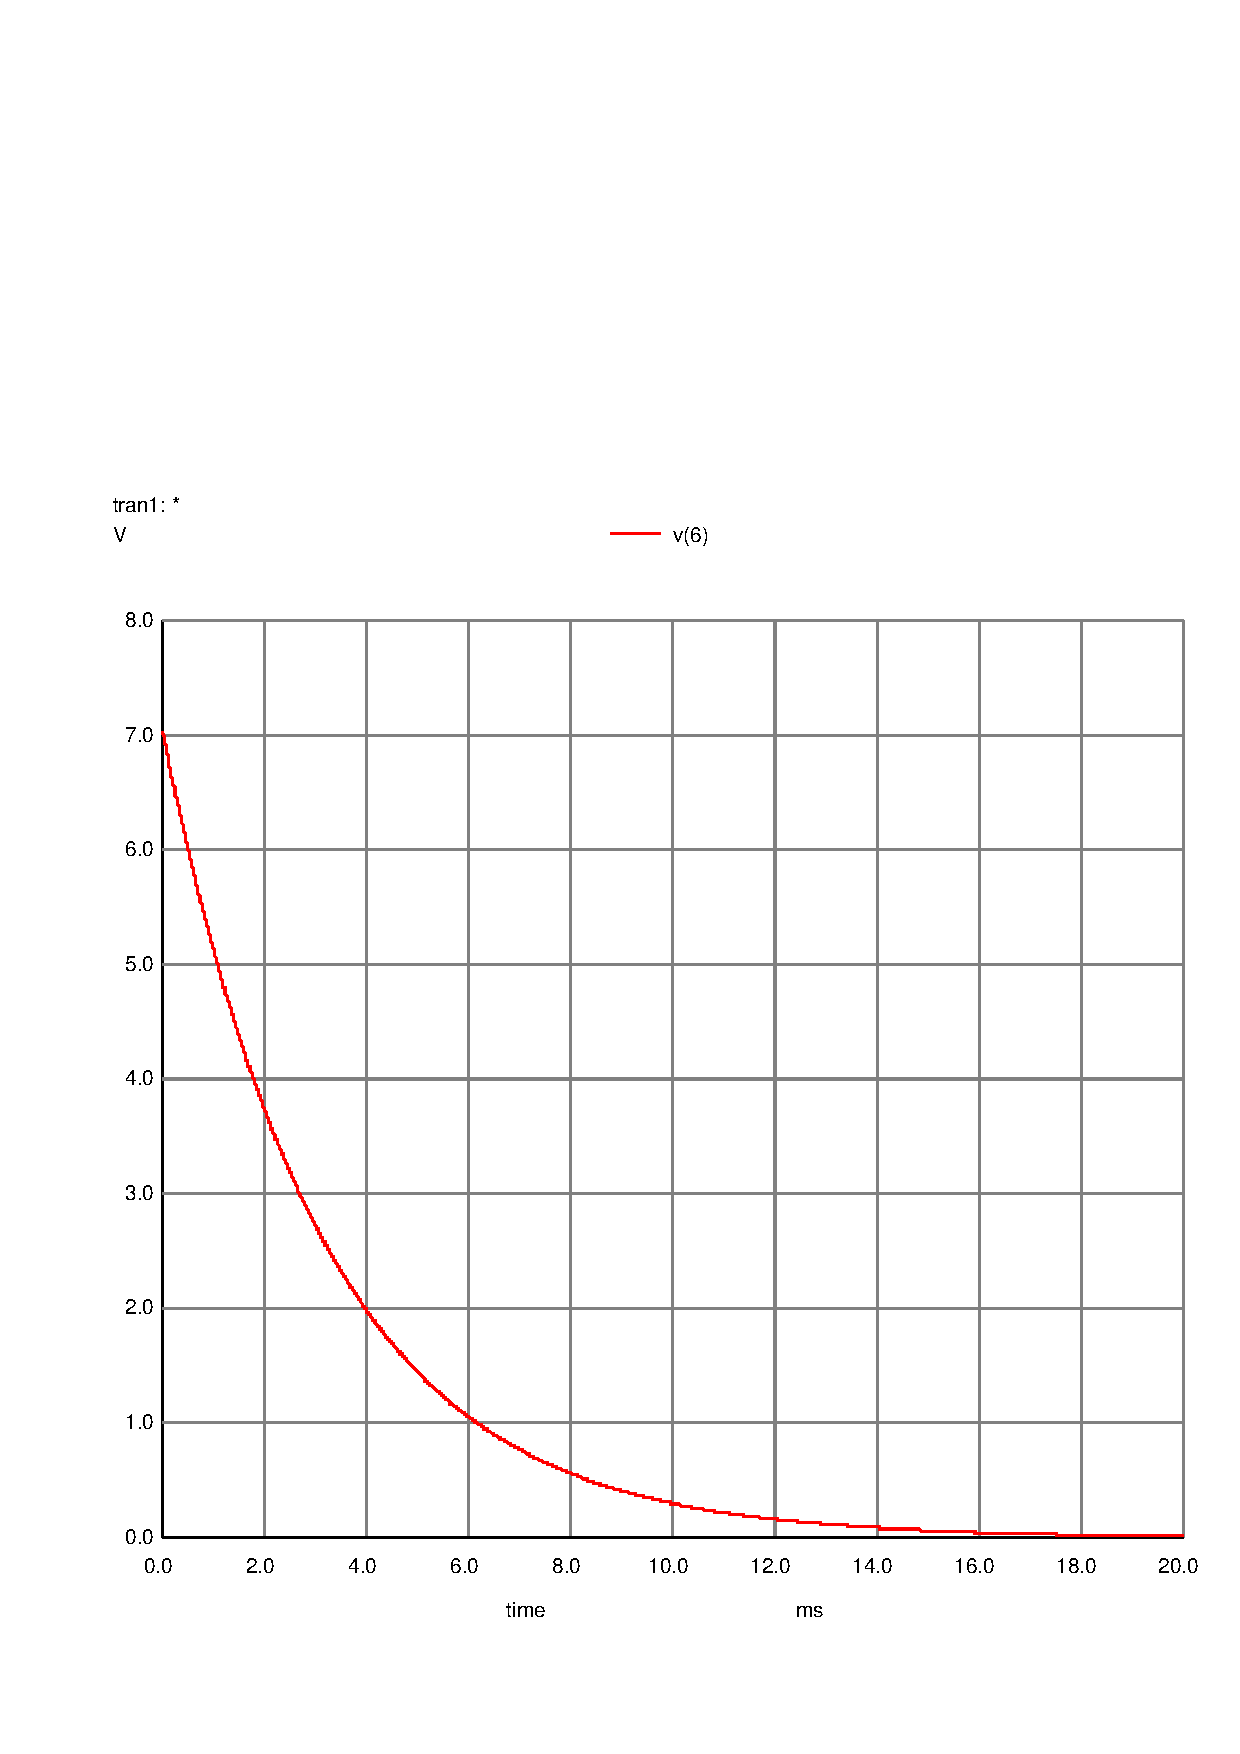
\includegraphics[width=\linewidth, clip]{../sim/trans.pdf}
    \label{fig:PStime}
  \end{subfigure}
  \begin{subfigure}{0.23\textwidth}
    \includegraphics[width=\linewidth, clip]{../mat/v6natural.png}
    \label{fig:PSciclo}
  \end{subfigure}

  \caption{\small Graphs of the natural solution of $v_6(t)$. Simulation on the left, theoretical analysis on the right.}
  \label{maquina}
\end{figure}

Looking at the graphs, the exactness is unquestionably clear. Therefore we can conclude that using Ngpice’s transient analysis is equivalent
to solving the first order differential equation given by theoretically analyzing the circuit. That equation leads to the natural solution of $v_6$, as in \ref{2.3}.


%%%%%%%%%%%%%%%%%%%%%%%%%PONTO 4%%%%%%%%%%%%%%%%%%%%%%%%%%%%%%%%%%%%%%%%%%%%%%
\subsection{The Final Total Solution} \label{3.4}

Simulating the total solution (sum of the natural and forced solutions) we simulate the transient solution and obtain the graphic bellow:
\begin{figure}[h]
  \centering
  \begin{subfigure}{0.23\textwidth}
    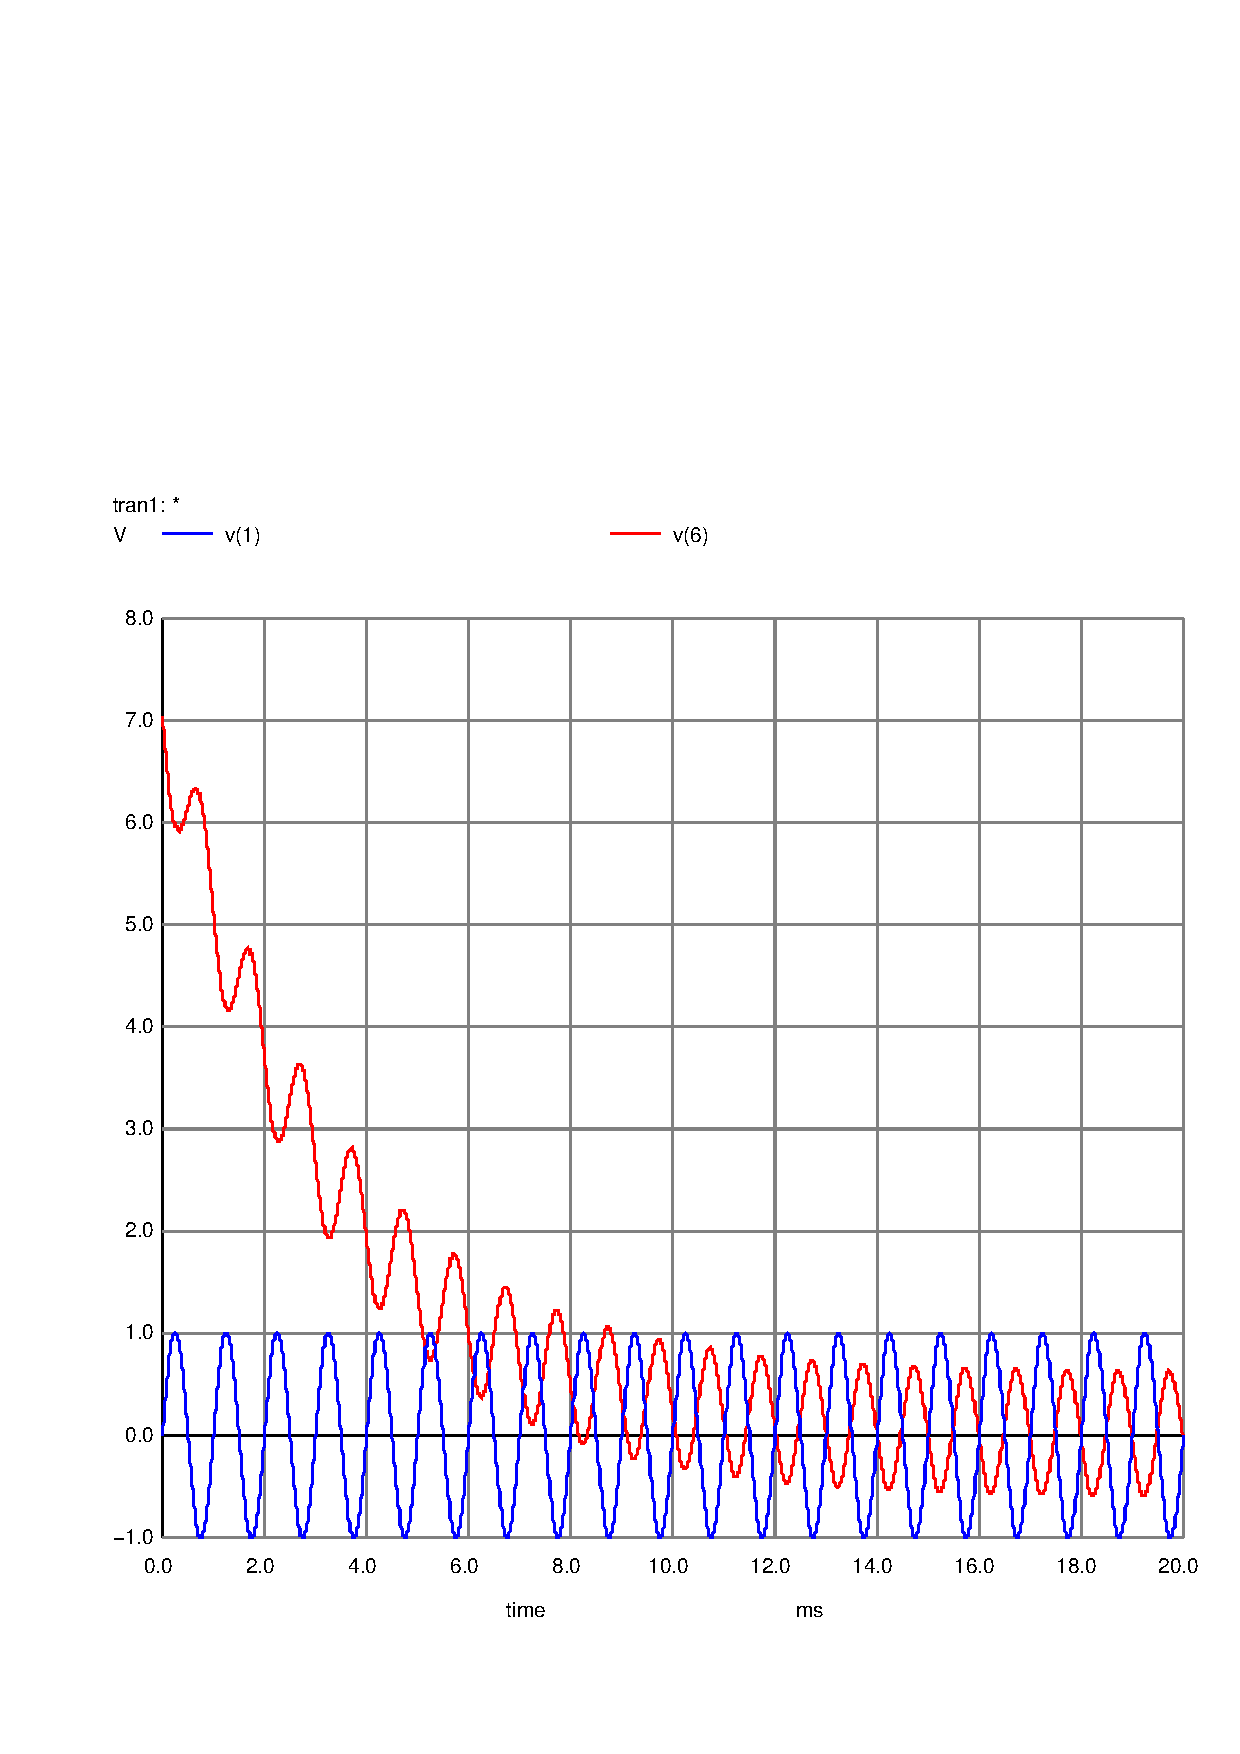
\includegraphics[width=\linewidth, clip]{../sim/trans4.pdf}
    \label{fig:PStime}
  \end{subfigure}
  \begin{subfigure}{0.23\textwidth}
    \includegraphics[width=\linewidth, clip]{../mat/total.png}
    \label{fig:PSciclo}
  \end{subfigure}

  \caption{\small Graphs of the total transient solution of $v_6(t)$ and $v_s(t)$. Simulation on the left, theoretical analysis on the right.}
  \label{maquina}
\end{figure}

As in \ref{3.3}, both graphs are exactly the same from $t=0$ up until the end. Consequently, converting the phasors to real time functions
for f=1KHz, and superimposing the natural and forced solutions is equivalent to repeating \ref{3.3} with $V_s(t)$ as given in \ref{fig:circuit} and f=1kHz.

%%%%%%%%%%%%%%%%%%%%%%%%%PONTO 5%%%%%%%%%%%%%%%%%%%%%%%%%%%%%%%%%%%%%%%%%%%%%%

\subsection{The Final Total Solution for the frequency range $0.1Hz$ to $1MHz$}


Now we simulate both the frequency response of the voltage in node 6, of $V_c$ and of $V_S$ and the phase response of this voltages.

\begin{figure}[h]
  \centering
  \begin{subfigure}{0.23\textwidth}
    \includegraphics[width=\linewidth, clip]{../mat/Transmagnitude.pdf}
  \end{subfigure}
  \begin{subfigure}{0.23\textwidth}
    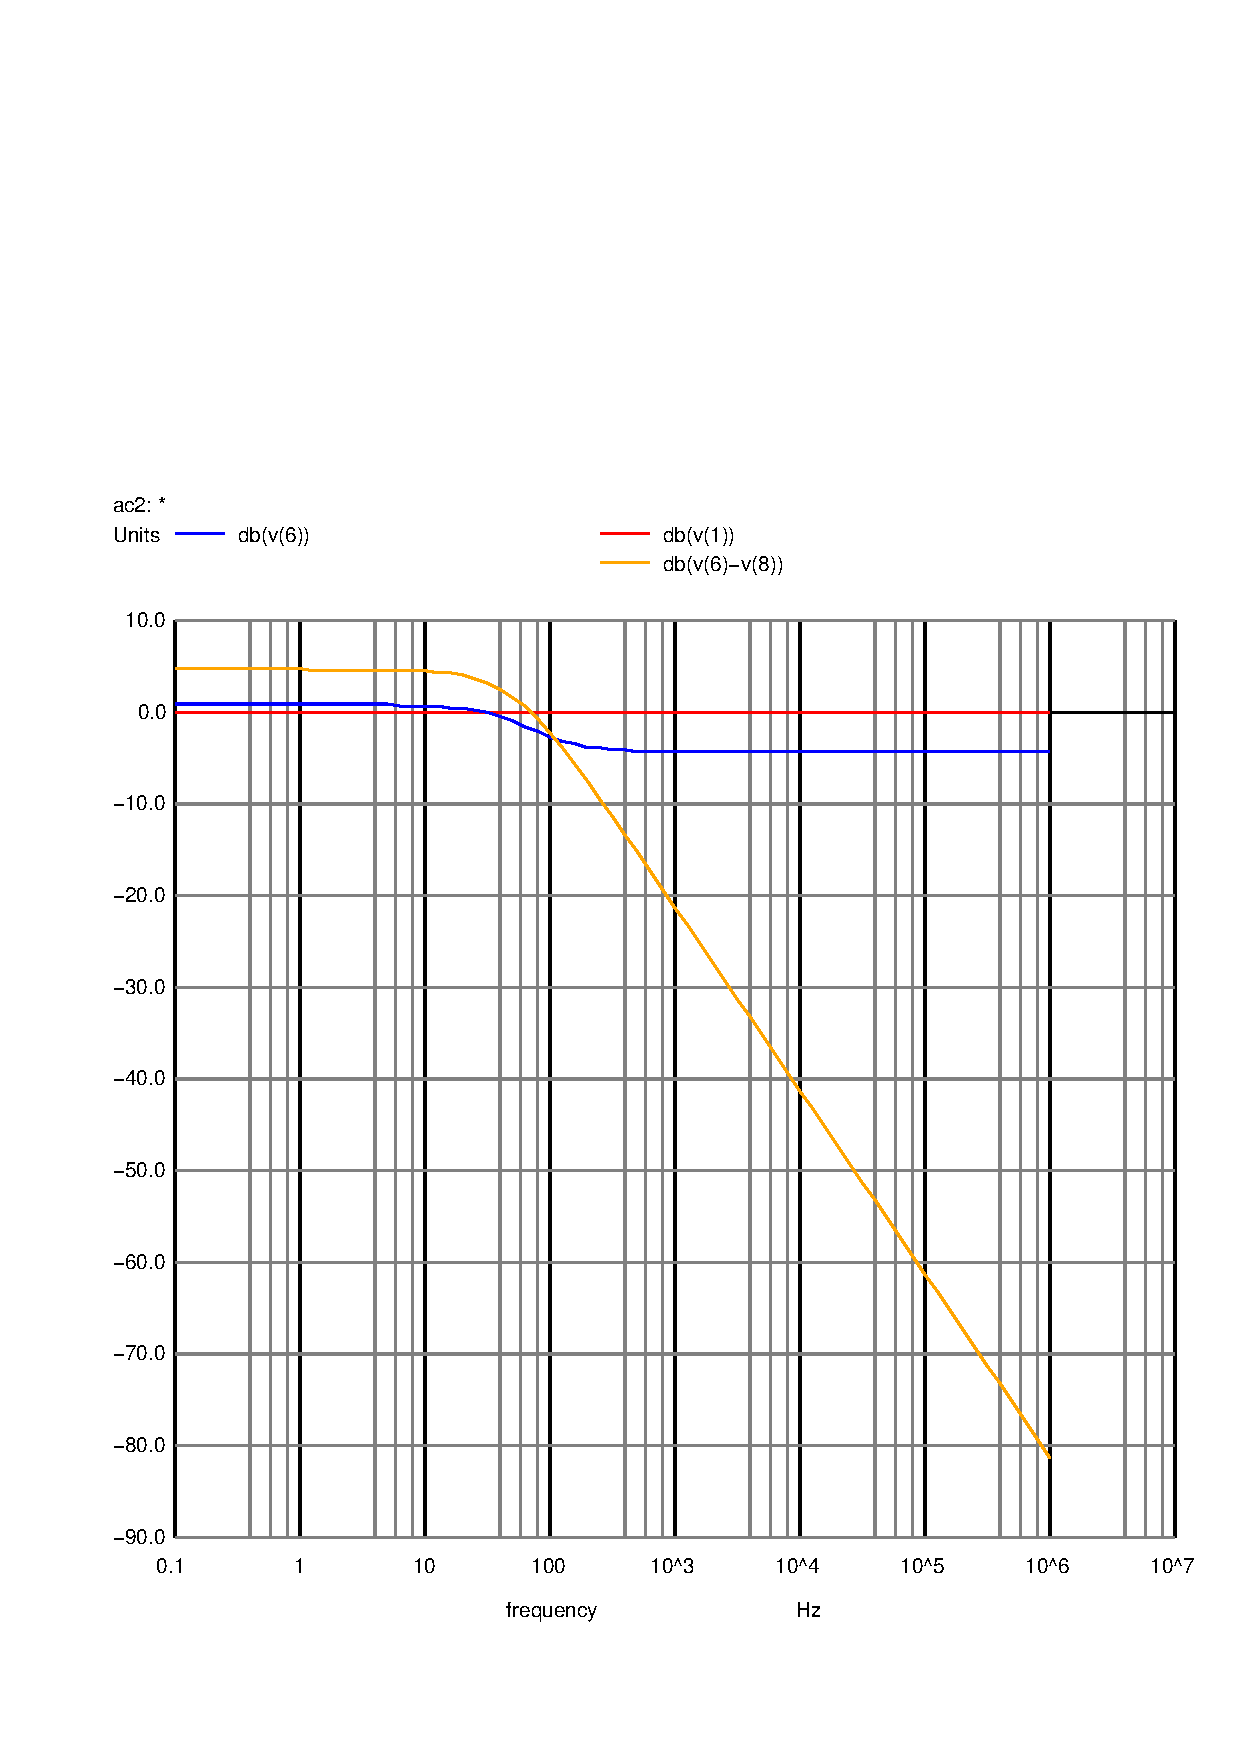
\includegraphics[width=\linewidth, clip]{../sim/mag.pdf}
  \end{subfigure}

  \caption{\small Representation of Total Solution in $[0,20]ms$}
\end{figure}

It is very noticeable that the graphs are the same in both the theorical analysis and the simulation.

\begin{figure}[h]
  \centering
  \begin{subfigure}{0.23\textwidth}
    \includegraphics[width=\linewidth, clip]{../mat/Transphase.pdf}
  \end{subfigure}
  \begin{subfigure}{0.23\textwidth}
    \includegraphics[width=\linewidth, clip]{../sim/phs.pdf}
  \end{subfigure}

  \caption{\small Representation of Total Solution in $[0,20]ms$}
\end{figure}

The phase reponse graphs are also the same.

We can conclude that both analysis methods are exact and can be confidently used in future projects.